\documentclass[11pt,letter]{article}

\setlength{\topmargin}{0in}
\setlength{\headheight}{0in}
\setlength{\headsep}{0in}
\setlength{\textheight}{8.5in}
\setlength{\oddsidemargin}{0in}
\setlength{\textwidth}{6.5in}

\usepackage{amsmath}
\usepackage{amsfonts}
\usepackage{amssymb}

\usepackage{epsfig}
\title{A Framework for Personalized Photograph Quality Assessment}
\author{
K. Armin Samii \\
ksamii@ucsc.edu
\and
Uliana Popov \\
uliana@soe.ucsc.edu}
\date{May 13, 2011}

\begin{document}
\maketitle
\begin{abstract}
Photograph quality assessment can help aid home users in managing their personal collections in several ways, including deleting low-quality images and browsing for high quality images. Recent research has aimed to automatically rate image quality, but such methods are not yet perfected. In this paper, we propose a framework for quickly developing and testing new features to accelerate the progress of this research. We have two types of features: \textit{high-level features} are subjective qualities which humans can easily answer, like saturation, exposure or blurriness; \textit{low-level features} are objective calculations which are produced algorithmically, like edge width or number of dark pixels. We use machine learning techniques to learn how each of these relate to image quality. Our model allows for a developer to easily train new features (both low-level and high-level), and for an end-user to personalize which high-level features are important.

\end{abstract}

\section{Problem Statement}
Before discussing the details of our solution, we present our problem in full.

A photographer wishes to automatically rate his pictures collection based on his personal preferences. There are several papers dedicated to solving this problem using machine learning\cite{springerlink:10.1007/11744078_23}\cite{springerlink:10.1007/978-3-642-10543-2_23}\cite{Yeh:2010:PPR:1873951.1873963}. To accelerate research in the area, we need to develop a framework for developers (researchers) to quickly train new features extracted from photographs.

There are two audiences we are trying to serve in this work: (1) the photographer using the application, and (2) the developer producing the application. In other words, we want to make it as easy as possible for the developer to serve the photographer.

To serve (1) the photographer, we want to allow him to choose which features he personally finds important (see Section \ref{abstraction}). To serve (2) the developer, we want to allow her to be able to add new features with ease (see Section \ref{easeofprogramming}). Figure \ref{fig:flowchart} visualizes these ideas.

First, a note on terminology: We make the distinction between \textit{low-level features} (ones that are computed, such as average edge width) and \textit{high-level features} (ones that are solely for human interpretation, such as blurriness).

\begin{figure*}[b!]
  \centering
    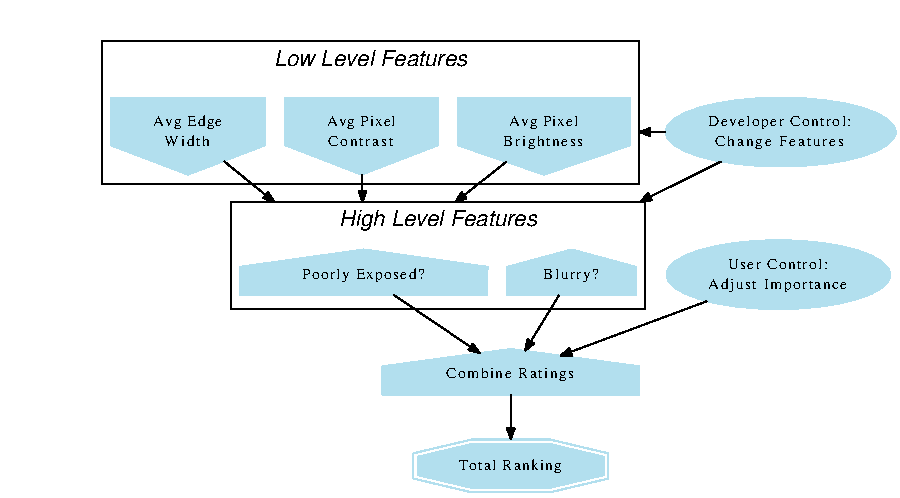
\epsfig{file=mlflowchart.pdf,width=14cm}
  \caption{An example flowchart. Here, the application computes three low-level features. All three combine to rate the two high-level features: blurriness and exposure. The developer controls which features are present. The photographer decides how to weight each high-level feature.}
  \label{fig:flowchart}
\end{figure*}

\subsection{Helping the Photographer Personalize Ratings}
\label{abstraction}
The photographer should not have to interpret the meaning of low-level features. Instead, we use high-level features as a layer of abstraction. It is easy for a photographer to understand the meaning of high-level features, but this presents the following two questions:

\begin{enumerate}
\item \textbf{How important is each high-level feature to the overall rating of a photograph?}

%This question is relevant to the photographer. As an example:

%Photographers Penny and Quinn want to automatically rate their photographs so they can ignore those with low ratings and save some time when browsing their collections.
For example: Photographer Penny takes pictures at concerts so she doesn't mind slightly underexposed images. Penny will decrease the default weight on the high-level "exposure" feature.

\item \textbf{How does each low-level feature affect the ranking of a high-level feature?}

%This  question is relevant to the developer. As an example:

For example: Programmer Pete calculates three low-level features per image: average width of edges, average pixel contrast, and average pixel brightness. He wants to use these low-level features to see if an image is blurry or poorly exposed.
\end{enumerate}

\subsection{Helping the Developer Make Progress}
\label{easeofprogramming}
The Developer will want to add more features as research progresses. There are two types of features which can be added:
\begin{enumerate}
\item \textbf{Adding low-level features}

Say Programmer Pete finds a new way to measure blur levels in an image. He should be able to insert this feature into the program with ease. The photographer would be unaware of any changes other than an improvement in accuracy.

\item \textbf{Adding high-level features}

Say Programmer Pete decides that Saturation is important. Then he will want to see just how much saturation is relevant to image quality. The end-user photographers will be aware of this new change, and can adjust the high-level weights accordingly.
\end{enumerate}

\section{Introduction}
To solve the problem presented, one might try to directly train low-level features to rate image quality. However, photograph quality is highly subjective and this approach does not allow a photographer to personalize the importance of each feature.

So instead, one might try to compute high-level features directly and allow the photographer to personalize the importance this way. However, this method risks using a poor algorithm to calculate a high-level feature, and thus sacrifices accuracy.

We thus propose a method which separately trains low-level and high-level features. This method allows (1) the photographer to personalize each high-level feature's importance, and (2) the developer to have multiple low-level calculations to rate each high-level feature. Further, the developer can (3) dynamically change which features are used.

To answer the first question presented in Section \ref{abstraction}, we use a Logistic Regression machine learning model. This allows for the photographer to adjust the importance of each feature without retraining the model. For the second question, we use the more accurate model of Support Vector Machines, because we do not need to reweight the low-level features. When the developer adds a new feature, one or both of these must get retrained. These methods are described in detail in Section \ref{methods}. The high-level features for the images in the training set are labeled by surveying Amazon Mechanical Turk\footnote{http://www.mturk.com} users (Turkers).

\section{Related Work}
Tong and Chang\cite{Tong:2001:SVM:500141.500159} use Support Vector Machines to search a database of images quickly by choosing images that are visually similar, which abstracts the features from the user completely.

The Personalized Photograph Ranking and Selection System\cite{Yeh:2010:PPR:1873951.1873963} computes high-level features directly and uses ListNet\cite{Cao:2007:LRP:1273496.1273513} to find a ranking. However, this does not allow for the training of several low-level features to produce a single high-level feature, which can increase the overall accuracy.

\section{Data}

There are two sets of data used, both of which are learned independently.

\subsection{User-Produced Data}
\label{turkdata}
The initial set of data was produced by giving Turkers a simple statement for each high level feature, and asking if they agreed. Our primary ground-truth statement for each image is:

``This image is high quality.''

We present this to five Turkers and ask them to choose one of three options:

\begin{itemize}
\item ``Agree'' (+1 point)
\item ``Neutral'' (+.5 points)
\item ``Disagree'' (+0 points)
\end{itemize}
The points are then averaged across the five Turkers' responses to obtain a final score.

We repeat this process for each high level feature, with statements such as ``This image is in focus'' and ``This image is well-exposed.'' The data then looks like:

\resizebox{12cm}{!}{
\begin{tabular}[t]{| c || c || c | c | c | l | }
 \hline
 & High Quality & In focus & Well exposed & Good saturation & \ldots \\ 
 \hline
Image 1 & .5 & .3 & 1 & .8 & \ldots \\ 
 \hline
Image 2 & .1 & .2 & .4 & .4 & \ldots \\ 
 \hline
\vdots & \vdots & \vdots & \vdots & \vdots & $\ddots$ \\
 \hline
\end{tabular}
}

\\
\\

In this way, the primary rating for an image is learned indirectly through a logistic regression of each of the other high-level features.

\subsection{Application-produced data}
The developer chooses which low-level features to calculate. Each calculation is used in a Support Vector Machine to get rankings of each high-level feature.

\section{Training Methods}
\label{methods}

There are two steps to the learning process. First, we learn the importance of each high-level feature on the overall image rating. Then, we learn how each low-level feature affects each high-level feature.

%We keep a held-out test set to recalculate the learning parameters when the developer adds a feature. When a new high-level feature is added, we ask Turkers to rank an image based on that feature. When a low-level feature is added, the parameters of each of the SVMs are updated.

\subsection{Learning High-Level Features}
We use a logistic regression to train each high level feature. For this, we do not take into account any low-level features. The error function is defined as:
\[
E=\displaystyle\sum\limits_{i=0}^N R_i-Z_i
\]
Where $E$ is the error, $N$ is the number of images in the training set, $R_i$ is the overall rating obtained from Turkers for image $i$, and $Z_i$ is as follows:
\[
Z_i=\displaystyle\sum\limits_{f=0}^M w_f \cdot r_{i,f}
\]
Where $M$ is the number of high-level features, $w_f$ is the weight of feature $f$, and $r_{i,f}$ is the Turkers rating of feature $f$ on image $i$.


\section{Progress thus far [informal]}
So far, we have gathered several hundred data points for two high-level features. We have increased the speed of previously written code to allow for several dozen images to be processed in a minute (as opposed to about 2 minutes per image previously).

We have implemented Support Vector Machines into our code and it is working on a small test set. We have a mostly-completed framework for dynamically changing high- and low-level features. No progress has been made on determining the weights of each high-level feature (for logistic regression).

We should note that we talk about our work as if the project were completed. It is not.


\section{Results [informal]}
We have a test set of several hundred images that we expect our application will rank highly, and another test set of several hundred blurry images that we expect to rank poorly. We will measure how much better we perform on blur detection after implementing machine learning techniques (we have accuracy results from before this paper). This does not take into account user preferences or ease of use of our framework.

%UUU. I'd talk here about the evaluation of the results, rather than about different / hard-to-understand data sets. 
% we can say that we will use the corelation or standard deviation to measure our success rate.

\bibliographystyle{plain}
\bibliography{README_BIB}

\end{document}
